Air pollution is the leading environmental health risk in many areas around the world affecting both the human population and ecology.
The effects of air pollution to the general population range from chronic to less severe health impacts, and reduced growth rates of vegetation due to air pollution results in economic losses running into billions of euros per year \citep{AQEU:2015}.
Moreover, air pollution has been labelled as carcinogenic by the International Agency for Research on Cancer \citep{IARC:2013}.
Due to these impacts, many governed areas introduced legislation designed to reduce concentrations of many air pollutants.

%Air pollutants can be emitted directly into the atmosphere (\emph{primary pollutants}) or formed from the chemical reactions of other pollutants (\emph{secondary pollutants}).
Tropospheric ozone (\ce{O3}) and particulate matter (PM) are the most problematic air pollutants over Europe with up to $98$ and $93$~\% of Europe's urban population exposed to concentrations of ozone and PM above the WHO guidelines \citep{AQEU:2015}.
Furthermore, in 2011 the EU ozone target value for human health (the EU does not currently have a  limit value for ozone) was exceeded in $65$~\% of the EU member states and Europe's ozone target value for vegetation was exceeded in $27$~\% of the EU-28 agricultural areas \citep{AQEU:2013}.

Reducing atmospheric concentrations of tropospheric ozone is a complex problem as ozone is not directly emitted into the troposphere.
Tropospheric ozone is produced from the reactions of nitrogen oxides \mbox{(\ce{NO_x}~$\equiv$~NO + \ce{NO2})} and volatile organic compounds (VOCs) in the presence of sunlight \citep{Atkinson:2000}.
Moreover, the photochemical nature of ozone production leads to a strong influence of meteorological variables, such as temperature and wind speed, on ozone production \citep{Jacob:2009}.

Air quality (AQ) models are an important tool for understanding ozone pollution and for predicting future air quality.
There are many AQ models available for investigating ozone pollution with different scales and dimensions depending on the scope of the modelling experiment.
Accurately representing the complexity of ozone production, such as emissions, atmospheric chemistry, meteorology and atmospheric transport, in a computationally efficient model is an ongoing challenge for the modelling community \citep{Russell:2000}.

Model intercomparison projects (MIPs) compare the outputs from different models, typically showing differences in tropospheric ozone due to differing representations of key processes.
For example, the ACCMIP (Atmospheric Chemistry and Climate Model Intercomparison Project) showed different magnitudes of future ozone burden in the same region \citep{Young:2013}.
The CCMI (Chemistry Climate Model Initiative) aims to investigate differences in the representation of chemistry, emissions and transport processes between models to understand the differences between predictions from global models \citep{Eyring:2013}.

Detailed process studies are key to understanding differences between model representations which could lead to differences in simulated ozone levels.
This thesis determines the effects of different representations of VOC degradation chemistry, VOC emissions and the effects of temperature on ozone production.
This assessment should be beneficial to the wider modelling community in understanding potential differences between model outputs and improving the current suite of models.

\section{Ozone} \label{s:ozone}
%atmospheric O3 with budget, lifetime, stratospheric & tropospheric ozone
Ozone is a atmospheric gas found in the stratosphere and troposphere, however its atmospheric effects are very different in these regions.
About 90~\% of the atmospheric ozone is present in the stratosphere with a peak mixing ratio of about $12$~ppm \citep{Seinfeld:2006}.
Stratospheric ozone absorbs the sun's ultraviolet radiation with wavelengths between $280$ and $315$~nm.
Since excess UV radiation may cause as skin cancer, cataracts and a suppressed immune system in humans, and can also damage land and aquatic ecosystems \citep{WMO:2010}, the absorption of UV radiation by stratospheric ozone is extremely important. 

In contrast, tropospheric (or surface) ozone is both a pollutant and a greenhouse gas. 
Increased levels of tropospheric ozone are harmful to humans, plants and other living systems. 
High ozone exposure may lead to pulmonary problems in humans and can decrease both crop yields and forest growth \citep{WMO:2010}. 

Globally, tropospheric ozone is mainly formed via photochemical production from the reactions of VOCs and \ce{NO_x}, described in Sect.~\ref{s:ozone_chemistry}.
Although surface ozone concentrations are also influenced by meteorology and atmospheric transport.
For example, a spring-time peak in tropospheric ozone concentrations is common in the mid-latitudes of the Northern Hemisphere originally attributed to transport of ozone from the stratosphere into the troposphere via the Stratosphere-Troposphere Exchange (STE) \citep{Monks:2000}.
However, ozone transported via STE rarely influences surface ozone levels \citep{Lelieveld:2000} and the spring maximum is due to the photochemical reactions occuring in the Northern Hemisphere spring after the buildup of reservoir species over winter \citep{Penkett:1986}.
These reservoir species are oxidised at a faster rate due to the increase in temperature, moisture and sunlight in spring.

Understanding the intracacies of surface ozone pollution requires a combined effort from the modelling, observational and chemical kinetic communities -- called the ``three-legged stool'' approach by \citet{Abbatt:2014}.
Modelling of ozone production helped in understanding the complexity of atmospheric chemistry, such as the non-linear relationship of ozone production with precursor (VOC and \ce{NO_x}) emissions.
Modelling studies attempt to reproduce observational trends of surface ozone and model predictions may inspire the set-up of new observational studies.
Chemical kinetic studies performed by laboratories give insights to missing or incorrect representations of atmospheric chemistry which may be included in updated models.

This thesis focuses on the representation of VOC degradation chemistry, VOC emissions and the ozone-temperature relationship within models and the influence on ozone production.
The state of the art knowledge of ozone production chemistry is outlined in Sect.~\ref{s:ozone_chemistry}, while sources of emissions of ozone precursors are described in Sect.~\ref{s:precursor_emissions}.
Finally, the effects of meteorology, in particular temperature, on ozone production is presented in Sect.~\ref{s:meteo_ozone}.
For the rest of this thesis, ozone shall refer to tropospheric ozone.

%The STE is driven by the Brewer-Dobson circulation \citep{Brewer:1949, Dobson:1956}, a relatively slow circulation (weeks to months) due to planetary wave disturbances in the troposphere \citep{Haynes:1991}.
%The circulation causes air to move downward from the stratosphere into the troposphere at the mid and high latitudes balanced by upward exchange at the tropics. 
%The STE also has a seasonal variability where the maximum transport occurs during spring \citep{Appenzeller:1996}, due to the increase in altitude of the tropopause - the boundary level between the troposphere and the stratosphere - which moves stratospheric air into the troposphere. 

%%metereology impacts 
%Tropospheric \ce{O3} is not only impacted by emission levels, it is also affected by meteorological variables such as temperature, number of hours of sunshine and wind as these impact transport, dry and wet deposition rates and also chemical reaction rates \citep{Hess:2009}.
%Meteorology influences both regional and global \ce{O3} \citep{Hess:2009}, climate patterns such as El Ni\~{n}o are also known to impact \ce{O3} levels in certain areas \citep{Sudo:2001}. 
%The effects of meteorology on ozone production shall be presented in more detail in Sect.~\ref{s:meteo_ozone}.
%
%In general, there has been great effort to reduce emissions of ozone precursors from anthropogenic sources.
%For example, the emissions of non-methane VOCs (NMVOCs) over Europe have decreased by $20$~\% and emissions of \ce{NO_x} have decreased by almost $30$~\% from 2004 levels.
%Despite these reductions in ozone precursors, up to $98$~\% of Europe's urban population are exposed to levels of ozone exceeding the WHO guidelines \citep{AQEU:2015}.

\section{Ozone Chemistry} \label{s:ozone_chemistry}
Ozone absorbs UV radiation producing either ground-state atomic oxygen (\ce{O(^3P)}) or excited singlet (\ce{O(^1D)}) oxygen atoms.
\begin{rxnarray}
    \ce{O3 + h\nu} & \rightarrow \ce{O2 + O(^3P)} \label{r:O3_hva} \\
    \ce{O3 + h\nu} & \rightarrow \ce{O2 + O(^1D)} \label{r:O3_hvb} 
\end{rxnarray}
Ground-state oxygen quickly reacts with oxygen to reform ozone.
\begin{rxnarray}
    \ce{O(^3P) + O2} & \xrightarrow[]{\text{\tiny{M}}} \ce{O3} \label{r:O_O2}
\end{rxnarray}
Thus there is no net loss or production of ozone through \eqref{r:O3_hva} and \eqref{r:O_O2}.
\ce{O(^1D)} may collide with \ce{N2} or \ce{O2} (represented as M in chemical reactions) stabilising to the ground-state.
\begin{rxnarray}
    \ce{O(^1D)} & \xrightarrow[]{\text{\tiny{M}}} \ce{O(^3P)} \label{r:O1D_M} 
\end{rxnarray}
This process again leads to a null cycle with ozone destruction balanced by production.
However, \ce{O(^1D)} can also react with water vapour producing two hydroxyl (OH) radicals.
\begin{rxnarray}
    \ce{O(^1D) + H2O} & \rightarrow \ce{2 OH} \label{r:O1D_H2O}
\end{rxnarray}

The OH radical is a highly reactive chemical species reacting with almost all trace chemical species in the troposphere but not relatively inert species such as \ce{N2} or \ce{O2}.
OH is primarily produced via \eqref{r:O1D_H2O} and is also catalytically produced during the degradation of VOCs.
These sources of OH together lead to a relatively high daytime concentration of OH of the order of  $10^6$~molecules~cm$^{-3}$.
\citep{Seinfeld:2006, Monks:2005}

The initial oxidation of VOCs by OH sets off a reaction chain which may lead to net production or loss of ozone depending on the atmospheric conditions.
For example, when carbon monoxide (CO) reacts with OH in the presence of oxygen, carbon dioxide and the hydroperoxy (\ce{HO2}) radical are formed.
In polluted areas with high-\ce{NO_x} concentrations, \ce{HO2} readily reacts with nitrogen oxide (NO) which regenerates OH and produces nitrogen dioxide (\ce{NO2}).
\begin{rxnarray}
    \ce{CO + OH} & \xrightarrow[]{\ce{O2}} \ce{HO2 + CO2} \label{r:CO_OH} \\
    \ce{HO2 + NO} & \rightarrow \ce{OH + NO2} \label{r:HO2_NO}
\end{rxnarray}
Photolysis of \ce{NO2} produces ground-state atomic oxygen producing ozone via \eqref{r:O_O2}.  
\begin{rxnarray}
    \ce{NO2 + h\nu} & \rightarrow \ce{NO + O(^3P)} \label{r:NO2_hv} 
\end{rxnarray}
OH may also react with NO to produce nitrous oxide (HONO), which rapidly photolyses to return OH and NO.
\begin{rxnarray}
    \ce{OH + NO} & \rightarrow \ce{HONO} \label{r:OH_NO} \\
    \ce{HONO + h\nu} & \rightarrow \ce{OH + NO} \label{r:HONO_hv}
\end{rxnarray}
However, termination of OH and \ce{NO2} regeneration occurs when OH reacts with \ce{NO2} as nitric acid (\ce{HNO3}) is formed and \ce{HNO3} may be removed through deposition processes.
\begin{rxnarray}
    \ce{NO2 + OH} \rightarrow \ce{HNO3} \label{r:NO2_OH}
\end{rxnarray}

In the low-\ce{NO_x} conditions away from polluted areas, OH and \ce{HO2} are interconverted through reactions with ozone.
\begin{rxnarray}
    \ce{OH + O3} & \rightarrow \ce{HO2 + O2} \label{r:OH_O3} \\
    \ce{HO2 + O3} & \rightarrow \ce{OH + 2 O2} \label{r:HO2_O3}
\end{rxnarray}
OH and \ce{HO2} may also react in a termination reaction producing water vapour and oxygen.
\begin{rxnarray}
    \ce{HO2 + OH} \rightarrow \ce{H2O + O2} \label{r:HO2_OH}
\end{rxnarray}
Other termination reactions involve combination reactions of \ce{HO2} radicals producing hydrogen peroxide (\ce{H2O2}).
\begin{rxnarray}
    \ce{HO2 + HO2} & \rightarrow \ce{H2O2} \label{r:HO2_HO2}
\end{rxnarray}
Hydrogen peroxide may be removed through deposition \citep{Gunz:1990} but may also be a temporary sink for the odd-oxygen species OH and \ce{HO2}, represented as \ce{HO_x}.
\begin{rxnarray}
    \ce{H2O2 + h\nu} & \rightarrow \ce{2 OH} \label{r:H2O2_hv} \\
    \ce{H2O2 + OH} & \rightarrow \ce{HO2 + H2O} \label{r:H2O2_OH}
\end{rxnarray}
In summary, the secondary degradation of CO produces ozone in high-\ce{NO_x} conditions while in low-\ce{NO_x} conditions ozone is destroyed.
\citep{Seinfeld:2006, Monks:2005}

The secondary degradation of higher VOCs has similar features to that of CO.
Methane (\ce{CH4}) with a mixing ratio of about $1.7$~ppmv is the most abundant VOC in the troposphere.
The reaction of methane with OH, in the presence of \ce{O2}, produces the methyl peroxy radical (\ce{CH3O2}) -- the simplest organic peroxy radical (\ce{RO2}).
\begin{rxnarray}
    \ce{CH4 + OH} \xrightarrow[]{\ce{O2}} \ce{CH3O2 + H2O} \label{r:CH4_OH}
\end{rxnarray}
Similar to CO oxidation, the level of \ce{NO_x} conditions play a crucial role in the fate of \ce{CH3O2} and whether ozone is produced or destroyed, this is depicted graphically in Fig.~\ref{f:CH4_oxidation}.
\begin{figure}[t]
    \begin{center}
        \caption[Methane degradation pathways]{Methane degradation pathways in low-\ce{NO_x} and high-\ce{NO_x} conditions. Taken from \citet{Monks:2005}.}
        \includegraphics[width = 0.1\textwidth]{CH4_degradation}
        \label{f:CH4_oxidation}
    \end{center}
\end{figure}

The general types of secondary degradation products formed during the degradation of methane can be extended to more complex non-methane VOCs (NMVOCs).
The initial oxidation of an NMVOC may not only occur by reaction with OH.
Unsaturated VOCs, such as alkenes, may also react with ozone while photolysis is a primary degradation pathways for carbonyl species.
While during the night-time, reaction with the nitrate (\ce{NO3}) radical is typically more important than OH-oxidation due to the relatively higher concentrations of \ce{NO3} during the night-time.

\begin{rxnarray}
    \ce{VOC + OH / NO3 / O3 / h\nu} & \xrightarrow[]{\ce{O2}} \ce{RO2} \label{r:VOC_init} 
\end{rxnarray} 
\begin{figure}[t]
    \begin{center}
        \caption[Schematic of general secondary degradation of VOCs]{Schematic diagram outlining general pathways of the secondary degradation of an emitted VOC.}
        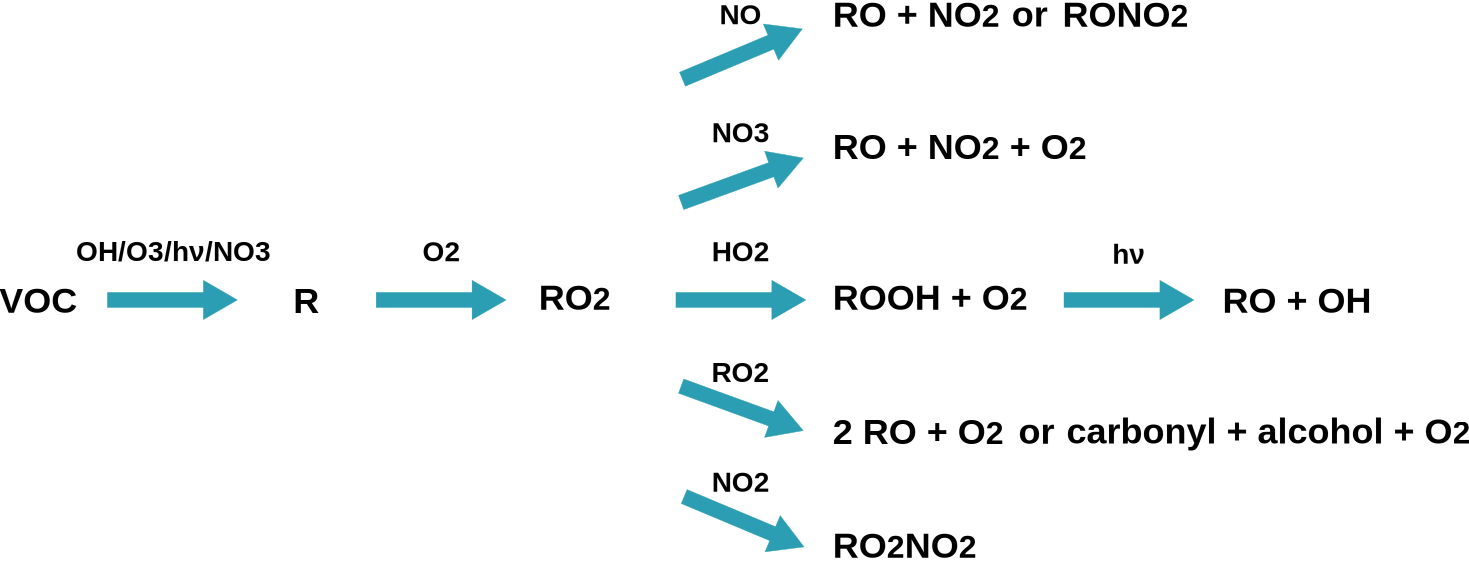
\includegraphics[width = \textwidth]{VOC_degradation}
        \label{f:VOC_reaction}
    \end{center}
\end{figure}

Figure~\ref{f:VOC_reaction} represents a general and simplified reaction scheme for VOCs in the troposphere. 
%The reaction of a VOC with OH forms an alkyl or substituted alkyl radical (R) which in the presence of \ce{O2} produces alkyl peroxy radicals (\ce{RO2}).
The initial oxidation of an NMVOC leads to the formation of \ce{RO2} radicals.  
Similar to CO and \ce{CH4} degradation, the fate of the peroxy radicals determines whether net loss or production of ozone occurs.
\begin{rxnarray}
    \ce{RO2 + NO} & \xrightarrow[]{\text{M}} \ce{RONO2} \label{r:RO2_NOa} \\
    \ce{RO2 + NO} & \rightarrow \ce{RO + NO2} \label{r:RO2_NOb} \\
    \ce{RO2 + NO2} & \xrightleftharpoons[]{\text{M}} \ce{RO2NO2} \label{r:RO2_NO2} \\
    \ce{RO2 + NO3} & \rightarrow \ce{RO + NO2 + O2} \label{r:RO2_NO3} \\
    \ce{RO2 + HO2} & \rightarrow \ce{ROOH + O2} \label{r:RO2_HO2} \\
    \ce{RO2 + RO2} & \rightarrow \ce{2RO + O2} \label{r:RO2_RO2a} \\
    \ce{RO2 + RO2} & \rightarrow \ce{RCH(OH)R + RC(O)R + O2} \label{r:RO2_RO2b}
\end{rxnarray}
All reactions pathways of \ce{RO2} that produce \ce{NO2} while simultaneously recycling radicals can result in \ce{O3} formation due to \eqref{r:NO2_hv} and \eqref{r:O_O2}. 
Reaction with the \ce{HO2} radical forms a hydroperoxide (ROOH) which may either be removed from the system or photolyse to produce an alkoxy (RO) radical and OH.
The carbonyl and alcohol products resulting from reaction with other \ce{RO2} radicals will follow a similar sequence of reactions and hence can also produce further \ce{O3}. 
Thus the subsequent reactions of secondary degradation products, also called the secondary chemistry, of a VOC may lead to further production of ozone.

Reaction of \ce{RO2} with \ce{NO2} forms peroxynitrates (\ce{RO2NO2}) which are a temporary reservoir for \ce{RO2} and \ce{NO_x}.
The thermal decomposition rate of \ce{RO2NO2} is highly temperature dependent.
Hence, at lower temperatures \ce{RO2NO2} may build up and be transported away from the region of formation and re-release \ce{RO2} and \ce{NO2} downwind fuelling ozone production away from large sources of \ce{NO_x}.
This is one example of the dependence of ozone production on meteorological variables, a broader overview is given in Sect.~\ref{s:meteo_ozone}.

%The secondary degradation of the RO radical formed from many of the \ce{RO2} reactions proceeds through either decomposition, isomerisation or reaction with \ce{O2}. 
%The products that result from the reaction pathways depend on the parent VOC and this also determines the number of NO-to-\ce{NO2} conversions, eventually leading to \ce{O3} formation.

Another important reaction involving ozone in polluted regions is that of NO with \ce{O3}.
\begin{rxnarray}
    \ce{NO + O3} & \rightarrow \ce{NO2 + O2} \label{r:NO_O3}
\end{rxnarray}
Together with \eqref{r:NO2_hv} and \eqref{r:O_O2}, this is a very important null cycle of ozone production and destruction.
In polluted areas with high NO emissions or in the night-time when no photochemistry occurs, the concentration of ozone is limited by the rates of \eqref{r:NO_O3} and \eqref{r:NO2_hv}.

%The path that a NMVOC takes to reach the final degradation products of \ce{CO2} and \ce{H2O} depends on the type of NMVOC, radical concentrations, \ce{NO_x} concentration and other factors such as time of day and year. 

\subsection[VOC and NOx Chemistry]{VOC and \ce{NO_x} Chemistry} \label{ss:VOC&NOx}
\begin{figure}
	\begin{center}
        \caption[Ozone mixing ratios as a function of \ce{NO_x} and VOC]{Ozone isopleth plots for various initial mixing ratios of \ce{NO_x} and a VOCs. taken from \citet{Jenkin:2000}.}
        \includegraphics[width = \textwidth]{O3_isopleth}
		\label{f:O3_isopleth}
	\end{center}
\end{figure}
%balance of NOx & NMVOC for O3 production
One of the most important features of ozone production, briefly hinted at prevously, is the dependence of ozone levels on both VOC and \ce{NO_x}.
Figure~\ref{f:O3_isopleth}, from \citet{Jenkin:2000}, depicts the non-linear relationship between \ce{O3} mixing ratios as a function of VOC and \ce{NO_x} mixing ratios.  
This relationship can be divided into distinct regimes of ozone production: \emph{\ce{NO_x}-sensitive} (or \emph{\ce{NO_x}-limited}), \emph{\ce{NO_x}-saturated} (or \emph{VOC-sensitive}) and \emph{VOC-and-\ce{NO_x}-sensitive} regimes. 

The cause of the non-linear relationship is the pathways available to \ce{RO2}.
In the \ce{NO_x}-sensitive regime, the concentration of \ce{NO_x} is low compared to that of radicals hence radicals are more likely to react with other radicals. 
The most common reactions are bimolecular destruction \eqref{r:HO2_OH}, which removes radicals, or combination of radicals \eqref{r:RO2_HO2} into reservoir species that can re-release radicals.

Reactions between radicals do not directly lead to ozone production as little NO is converted to \ce{NO2}.
Thus increasing \ce{NO_x} would increase the number of NO to \ce{NO2} reactions by peroxy radicals leading to ozone production.
However, increasing VOC levels would not increase \ce{O3} production as increases the likelihood of radical descruction or combination reactions.

The \ce{NO_x}-saturated regime corresponds to high \ce{NO_x} concentrations where radicals will tend to react with \ce{NO_x}. 
Increased \ce{NO_x} levels will not increase \ce{O3} production due to an increase in nitric acid (\ce{HNO3}) formation \eqref{r:NO2_OH}.
Nitric acid is a sink for both OH and \ce{NO_x} removing OH which would otherwise react with emitted VOC to fuel further radical production.

The VOC-and-\ce{NO_x}-sensitive regime is characterised by \ce{O3} production being sensitive to both VOC and \ce{NO_x} levels. 
Morever, it is in this atmospheric regime that the maximum amount of ozone is produced and corresponds to the contour ridges in Fig.~\ref{f:O3_isopleth}.
The non-linear relationship can be thought of as a titration process between the amount of radicals and the \ce{NO_x} present in the atmosphere with the VOC-and-\ce{NO_x}-sensitive regime being the turning point \citep{Kleinman:1991, Kleinman:1994}.

This non-linear nature of the troposphere to ozone production makes controlling ozone levels particularly difficult.
The difficulty is exacerbated by the fact that regions can alternate between these regimes depending on the season, time of day etc.
Moreover, fresh emissions tend to occur in the \ce{NO_x}-saturated regime and through transport, the emissions are advected to VOC-and\ce{NO_x}-sensitive and even \ce{NO_x}-sensitive regions.

\subsection{Representing Atmospheric Chemistry in Models} \label{ss:chemistry_models}
The degradation of most VOCs is well-understood however for more complex VOCs the complete set of reaction pathways of all the secondary degradation products there are a great number of uncertainties. 
These uncertainties may be related to kinetic data, photolysis rates and in most cases the reaction products.

Any uncertainties in reaction pathways and degradation products also leads to uncertainties in estimating the amount of ozone produced during the degradation of a particular VOC \citep{Atkinson:2000}.
Representing this complex chemistry for each emitted VOC in a chemical transport model (CTM) is unrealistic.
Even if all the secondary degradation pathways and products were known for every VOC, a CTM would not be able to efficiently numerically solve the resulting differential equations.
Hence, CTMs use descriptions of atmospheric chemistry that lead to more computationally efficient models.

Not all representations of atmospheric chemistry used in a \emph{chemical mechanism} are prepared in the same way.
For a start, models that also numerically compute meteorology fields require very computationally efficient chemical mechanisms including around $150$ unique species while simpler box models can use chemical mechanisms having many thousands of species.
The simplification techniques used to represent the multitude of VOC and their degradation may lead to discrepancies in the estimations of ozone production.
We compare the ozone production from many reduced chemical mechanisms to a highly detailed chemical mechanism in Sect.~\ref{s:chemical_mechanism_results} and the research questions addressed in this study are framed in Sect.~\ref{s:research_questions}.
\todo{use Stockwell:2012 review}

\section{Emissions of Ozone Precursors} \label{s:precursor_emissions}
% NOx sources and quantities, weekend effect
\subsection[NOx]{\ce{NO_x}}
Emissions of \ce{NO_x} are mainly through anthropogenic activity.
In the year 2000, almost $52$~Tg~N were emitted with 65~\% through the many forms of fossil fuel combustion \citep{Seinfeld:2006}. 
Examples of fossil fuel combustion that releases \ce{NO_x} are transportation using diesel or petrol vehicles, industrial activities and domestic heating \citep{vonSchneidemesser:2015}.

Up to $95$~\% of \ce{NO_x} emissions from combustion are emitted as NO, which then is oxidised to form \ce{NO2} through \eqref{r:NO_O3} and \eqref{r:RO2_NOb}.
However, due to the increase in diesel vehicles and the implementation of diesel filters the fraction of emitted \ce{NO2} has increased.
\citet{Grice:2009} showed that over Europe, emissions of \ce{NO2} from diesel vehicles has increased from $8.6$~\% in 2000 to $12.4$~\% in 2004.

Despite the overwhelming majority of \ce{NO_x} emissions coming from human activities, there are many important natural sources of \ce{NO_x}.
Lightning and soils are also important sources of \ce{NO_x}, each source contributed about $10$~\% to global \ce{NO_x} emissions in 2000 \citep{Seinfeld:2006}.

\subsection{VOCs}
\subsubsection{Carbon Monoxide}
Carbon monoxide, CO, is emitted directly into the troposphere through combustion and industrial processes.
Another equally-important source of CO, is its chemical formation during the degradation of VOCs.
\citet{Hauglustaine:1998} estimated that globally $881$~Tg~yr$^{-1}$ of CO was produced from chemical oxidation of VOC while $1219$~Tg~yr$^{-1}$ of CO was directly emitted.

Oxidation of CO, through reaction with OH, is its major atmospheric sink and can lead to ozone production.
When the hydroperoxy radical (\ce{HO2}) reacts with NO, \ce{NO2} is formed which may produce ozone and OH is again recycled and available to further oxidise other chemical species.

The maximum possible yield of ozone from the degradation of a single molecule of CO occurs when each peroxy radical converts NO to \ce{NO2}.
In this case, a maxmimum of one molecule of ozone can be produced per molecule of CO oxidised.
In reality, this is never achieved as other reactions with the peroxy radicals occur however this is a very informative measure of the \emph{ozone production potential} of a species.

\subsubsection{Methane}
Emissions of methane are between $500$ and $600$~Tg~\ce{CH4}~yr$^{-1}$ with about $60$~\% of the emissions from anthropogenic sources.
The main anthropogenic sources of \ce{CH4} are agriculture, fossil fuels and biomass burning with agriculture contributing $60$~\% of the anthropogenically emitted methane.
Emissions from wetlands are the main natural source of methane emissions \citep{Kirschke:2013}.

Reaction with OH is the main sink of methane and this reaction is important for the concentration of OH in the troposphere.
With increased methane emissions, the concentration of OH will decrease via \eqref{r:CH4_OH} which would lead to a build of methane and other VOCs in the troposphere \citep{Holmes:2013}.

The secondary degradation of methane produces the methylperoxy radical \ce{CH3O2} as well as \ce{HO2} as well as CO.
Assuming that every peroxy radical converts NO to \ce{NO2} then methane degradation can produce a maximum five molecules of \ce{O3} per molecule of \ce{CH4} oxidised.
Methane (\ce{CH4}) has a lifetime of about $9$~years, significantly longer than all other VOCs.
Thus, methane influences ozone production on the global rather than the regional scale.  

\subsubsection{Non-Methane VOCs}
%VOCs, types of VOCs and source (A vs B)
A wide variety of non-methane VOC (NMVOC) are emitted from anthropogenic activities directly into the troposphere.
Solvent use, industry, fossil fuel burning and transportion are all major activities emitted NMVOCs of varying functional groups and carbon numbers.
The maximum number of molecules of \ce{O3} produced per degradation of an emitted NMVOC depends on the number of NO to \ce{NO2} conversions by the peroxy radicals formed during the degradation of the NMVOC.
This is highly dependent on the type of NMVOC and the number of carbons in the NMVOC.

Many NMVOCs emitted from anthropogenic sources are also hazardous to human health in their own right.
For example, benzene and formaldehyde are suspected carcinogens \citep{Laurent:2014}.
It is also worthwhile to note that the NMVOC thought to be the most hazardous to human health do not correspond to NMVOC that have a high ozone production potential.

Globally, \citet{Lamarque:2010} estimated that $130$~Tg~NMVOC were emitted from anthropogenic sources in the year 2000.
This amount is dwarfed by the total emissions from biogenic sources -- $1000$~Tg~NMVOC~yr$^{-1}$, almost eight times the amount of NMVOC emitted from anthropogenic sources \citep{Guenther:2012}.

Of the NMVOC emitted from vegetation, isoprene (\ce{C5H8}) dominates at the global scale however emissions of monoterpenes and sesquiterpenes are also significant.
There is typically overlap in the NMVOC species emitted from biogenic and anthropogenic sources. 
For example, isoprene has also been measured in the urban areas of London and Paris away from direct emission sources and since isoprene is a very reactive NMVOC it is unlikely to be transported from outside the area, there appears to be anthropogenic sources of isoprene \citep{vonSchneidemesser:2011}.
Also many small NMVOC that are typically emitted from anthropogenic sources, such as methanol and acetaldehyde, are also emitted from vegetation \citep{Guenther:2012}.

The NMVOC species emitted vary between types of vegetation -- some trees emit large amounts of isoprene while others do not.
Also, the quantity of NMVOC emissions from vegetation depends on atmospheric (such as, temperature and radiation) and biological variables (such as, leaf age and leaf area index).
Thus only regulation of NMVOC from anthropogenic sources is possible and drastic reductions in anthropogenic \ce{NO_x} are required to minimise the burden of the population to ozone pollution.
Areas dominated by biogenic NMVOC emissions and away from large \ce{NO_x} sources (\ce{NO_x}-sensitive regime) could lead net loss of ozone through direct reactions of ozone with many biogenic NMVOC and the net loss of radicals (discussed in Sect.~\ref{ss:VOC&NOx}).

\subsection{Representing VOC Emissions in Models}
%representation of VOC emissions in models using emission inventories
Representing the multitude of emitted VOCs, from either anthropogenic or biogenic sources is one of the major challenges of the modelling community.
Models use emission inventories that specify the type and quantity of VOCs emitted over a region or even the whole globe.
However, as hinted at, this is no easy task and emission inventories are one of the major sources of uncertainty of the model input \citep{Russell:2000}.

Emission inventories typically specify emissions for \ce{NO_x}, CO, \ce{CH4}, NMVOC as well as non-gas-phase emissions such as particulate matter.
Emissions are assigned to source sectors, called SNAP (Standardised Nomenclature for Air Pollutants) sectors, such as those listed in Table~\ref{t:SNAP}.
The rest of this section shall discuss specifications of NMVOC emissions from emission inventories.

\begin{table}
    \centering
    \caption[SNAP sectors in the TNO\_MACCIII]{SNAP sectors for anthropogenic emissions listed in the TNO\_MACCIII inventory \citep{Kuenen:2014}.}
    \begin{tabular}{cl}
        \hline \hline
        \textbf{SNAP Sector} & \textbf{Description} \\
        \hline \hline
        1 & Public Power \\
        2 & Residential Combustion \\
        34 & Industry \\
        5 & Fossil Fuel \\
        6 & Solvent Use \\
        71 & Road Transport: Gasoline \\
        72 & Road Transport: Diesel \\
        73 & Road Transport: Others \\
        74 & Road Transport: Evaporation \\
        75 & Road Transport: Wear \\
        8 & Non-road Transport \\
        9 & Waste \\
        10 & Agriculture \\
        \hline \hline
    \end{tabular}
    \label{t:SNAP}
\end{table}

%temporal profile of emissions
Emissions of both \ce{NO_x} and VOCs are not constant over the year, month or time of day.
In many regions, a noticible reduction in \ce{NO_x} emissions, due to reduced road transport, is noted during the weekend -- called the ``weekend-effect''.
The weekend-effect has implications on the ozone production during the weekend.
For example, ozone production is \ce{NO_x}-saturated during weekdays in San Joaquin Valley, California.
The reduction of \ce{NO_x} emissions during the weekend moves ozone production to the VOC-and-\ce{NO_x} sensitive regime, hence higher ozone levels are measured during the weekend \citep{Pusede:2014}.

Anthropogenic NMVOC emissions from the different SNAP sectors also have a temporal distribution.
Many SNAP sectors, such as industry and solvent use, have a reduction in emissions on weekends.
Transport emissions tend to peak during the morning and evening rush hours and emissions due to solvent have a strong diurnal cycle.
Residential combustion tends to be highest during the winter months and lowest during the summer \citep{Gon:2011}.

Emission factors are assigned to the emissions from SNAP categories to represent the temporal profiles within a model.
Biogenic VOC emissions are typically estimated using an algorithm including variables on which BVOC emissions are dependent.
MEGAN2.1 \citep{Guenther:2012} is commonly used by the modelling community to represent emissions from nature.
The MEGAN2.1 model utilised variables such as temperature and radiation levels which are calculated during model simulations and then fed into the MEGAN2.1 model to estimate BVOC emissions.

%emissions in models - lumping
One issue for the modelling community with using emission inventories for specifying NMVOC emissions is translating the listed emissions into the chemical species used by the chemical mechanism.
Emission inventories are not normally immediately available for use with a chemical mechanism which can lead to different modelling groups allocating the emission inventory input differently for the same chemical mechanism \citep{Carter:2015}.
Chemical mechanisms used in global and regional models cannot represent each NMVOC individually for reasons of computational efficiency thus many NMVOCs must be represented by the particular lumped (or aggregated) species of the chemical mechanism.
This translation into lumped species differs between chemical mechanisms (Sect.~\ref{ss:chemistry_models}).
The effect that lumping emissions of NMVOC into different chemical mechanism has on simulated ozone production is explored in this work in Sect.~\ref{s:EI_results}.

\section{Effects of Meteorology on Ozone Production} \label{s:meteo_ozone}
\begin{table}
    \centering
    \caption[Influence of meteorological variables on ozone production]{Influence of meteorological variables on ozone production, taken from \citet{Jacob:2009}.}
    \begin{tabular}{ll}
        \hline \hline
        \textbf{Meteorological Variable} & \textbf{Influence on Ozone} \\
        \hline \hline
        Temperature & Consistently positive \\
        Regional Stagnation & Consistently positive \\
        Wind Speed & Generally negative \\
        Mixing Depth & Weak or variable \\
        Humidity & Weak or variable \\
        Cloud Cover & Generally negative \\
        Precipitation & Weak or variable \\
        \hline \hline
    \end{tabular}
    \label{t:meteo_vars}
\end{table}

As the chemical processes of ozone production are photochemical in nature, meteorology has a significant influence on the amount of ozone produced.
The influence of meteorology on ozone production is particularly important for predicting air quality in a world under the effects of climate change and the effects changed weather systems would have.
Climate change is predicted to influence many meteorological variables that impact ozone production, Table~\ref{t:meteo_vars}, taken from \citet{Jacob:2009}, details the effects specific meteorological variables have on ozone production.

\subsubsection{Temperature}
Temperature is positively correlated with ozone in many areas.
\citet{Otero:2016} showed that temperature was the main driver of summertime ozone values over many areas of central Europe while \citet{Camalier:2007} correlated ozone with temperature over the Eastern US.
Interestingly only ozone pollution (higher values of ozone) and not background ozone, the ozone levels without the influence of anthropogenic emissions. is correlated with temperature \citep{Sillman:1995a}.

Temperature positively influences ozone levels directly in two ways: increasing the emissions of VOCs from vegetation and speeding up the rates of chemical reactions.
\citet{Pusede:2015} reviewed the chemical processes that exhibit temperature dependency and the relation of temperature on ozone production.
The production of radicals (OH, \ce{HO2}, \ce{RO2}) and temperature-dependence of organic reactivity strongly influence the production of ozone.
The shorter lifetime of peroxy nitrates at higher temperatures, increased radical production during VOC degradation, changes in emissions of both VOC and \ce{NO_x} and formation of alkyl nitrates \eqref{r:RO2_NOb} all exhibit temperature dependent influences on ozone production.

Despite many studies from an observational and regional modelling perspective correlating temperature with ozone production, there has been a lack of detailed process studies separating the direct effects of temperature on ozone.
Moreover, there are no attempts to tease the relative importance of the chemical processes listed in \citet{Pusede:2015} on ozone production.
The final part of this study addresses the whether higher emissions or faster chemistry is more important for ozone production and also which chemical processes are the most important for ozone production.
The results of this study are presented in Sect.~\ref{s:T-O3_results}.

\subsubsection{Humidity}
Humidity levels influences ozone production both positively and negatively.
When \ce{O^1D}, coming from ozone photolysis \eqref{r:O3_hvb}, reacts with water vapour \eqref{r:O1D_H2O}, the production of OH radicals leads to ozone loss.
However, the initiation of VOC degradation through reaction with OH can lead to ozone production as described in Sect.~\ref{s:ozone_chemistry}.
These competing effects of water vapour on ozone production leads to a weak correlation of ozone production with water vapour \citep{Jacob:2009}.

\subsubsection{Wind Speed and Stagnation}
High wind speeds transport ozone precursors away from their sources leading to a generally negative effect on ozone pollution over a region.
\citet{Doherty:2013} projected using a multi-model study that while climate change is expected to change large-scale atmospheric transport, model projections show that these have little influence on the spatial patterns of mean concentrations of ozone.

When low wind speeds are present over polluted urban areas stagnant conditions arise and these atmospheric conditions are highly correlated with increased ozone production over urban areas \citep{Jacob:2009}.
Typically stagnant conditions are also related to periods of high temperatures which may further fuel ozone production.
During periods of stagnant conditions, the ozone produced from the previous day (the ozone-lag) is not transported downwind, add the ozone production from emissions of ozone precursors and this leads to high ozone episodes \citep{Jacob:2009}.

\subsubsection{Mixing Height}
The effects of increased mixing heights of the planetary boundary layer (PBL) with the free troposphere are not so straightforward.
\citet{Dawson:2007} found that over the Eastern U.S., regions with low ozone are positively correlated with mixing height whereas regions with high ozone levels are negatively affected.
This spatial effect of mixing height on ozone production comes from whether the free troposphere ozone levels are higher or lower than the ozone levels within the PBL \citep{Jacob:2009}.
The study of \citet{Dawson:2009} showed that the predicted lower PBL heights coupled with stagnant conditions led to increased levels of ozone.
%Free troposphere ozone levels tend to be around $60$~pbv in the northern mid-latitudes \citep{Logan:1999}.

\section{Research Questions} \label{s:research_questions}
The overarching research question of this thesis is to determine detailed chemical processes affecting tropospheric ozone production.
This broad question is further focused on detailed modelling studies that bring out which chemical processes have the largest impact on tropospheric ozone production.
The focus of the study is further narrowed to look at the important chemical processes affecting ozone production under three different conditions that influence .

Firstly, AQ models have a choice in the representation of the chemistry, these chemical mechanisms are produced using different approaches which may impact on ozone production.
Furthermore, the scope of a modelling study (point, regional or global) may limit the choice of chemical mechanism to an extremely simplified version of the complex atmospheric chemistry detailed in Sect.~\ref{s:ozone_chemistry}.
Thus leading to the first research questions:
\begin{itemize}
	\item How do the simplification techniques used in different chemical mechanisms affect ozone production? 
    \item Does the choice of chemical mechanism impact predicted ozone production?
\end{itemize}

Secondly, the model inputs are critical for modelling studies and the specified inputs of NMVOC emissions are known to be a large source of uncertainty.
Emission inventories specify the NMVOCs emitted from different anthropogenic activities.
Different emission inventories are available to the modelling community and these may vary the speciations of different NMVOCs for the different sectors of anthropogenic activity.
We narrowed the focus to the solvent use sector, the sector with the largest percentage emissions, and used these different speciations to address the following questions:
\begin{itemize}
	\item What is the influence on predicted ozone production when using different speciations of emitted NMVOCs? 
    \item How does this influence change when using different chemical mechanisms?
\end{itemize}

Finally, meteorology influences the amount of ozone production with temperature being listed as the meteorological variable with the strongest positive correlation with ozone.
Temperature influences the amount of emissions from biogenic sources and also influences the reaction rates of chemical reactions.
These effects have been noted in many modelling and observational studies but not under varying \ce{NO_x} conditions that would lead to the different \ce{NO_x} regimes of the atmosphere.
\begin{itemize}
    \item Are temperature dependent emissions or temperature dependent chemical processes more important for ozone production with increasing temperature? 
    \item How is temperature dependent ozone production treated in different \ce{NO_x} regimes within a box model?
\end{itemize}

Chapter~\ref{c:methodology} details the methodology used to address these questions in greater detail.
The results from the separate studies and relevant publications are found in Chap.~\ref{c:papers}.
A broader discussion of the answers to the above research questions and their applications to the AQ modelling community are discussed in Chap.~\ref{c:conclusions}.
